%%%%%%%%%%%%%%%%%%%%%%%%%%%%% Define Article %%%%%%%%%%%%%%%%%%%%%%%%%%%%%%%%%%
\documentclass{article}
%%%%%%%%%%%%%%%%%%%%%%%%%%%%%%%%%%%%%%%%%%%%%%%%%%%%%%%%%%%%%%%%%%%%%%%%%%%%%%%

%%%%%%%%%%%%%%%%%%%%%%%%%%%%% Using Packages %%%%%%%%%%%%%%%%%%%%%%%%%%%%%%%%%%
\usepackage{ctex}
\usepackage{geometry}
\usepackage{graphicx}
\usepackage{pgfplots}
\usepackage{float}
\usepackage{minted}
\usepackage{hyperref}
\hypersetup{
  colorlinks=true,
  pdfstartview=Fit,
  pdfcreator={Shit},
pdfproducer={Big shit}}
%\usepackage{amssymb}
%\usepackage{amsmath}
%\usepackage{amsthm}
%\usepackage{empheq}
%\usepackage{mdframed}
%\usepackage{booktabs}
%\usepackage{lipsum}
%\usepackage{color}
%\usepackage{psfrag}
%\usepackage{bm}
%%%%%%%%%%%%%%%%%%%%%%%%%%%%%%%%%%%%%%%%%%%%%%%%%%%%%%%%%%%%%%%%%%%%%%%%%%%%%%%

% Other Settings

%%%%%%%%%%%%%%%%%%%%%%%%%% Page Setting %%%%%%%%%%%%%%%%%%%%%%%%%%%%%%%%%%%%%%%
\geometry{a4paper}

%%%%%%%%%%%%%%%%%%%%%%%%%%%%%%% Plotting Settings %%%%%%%%%%%%%%%%%%%%%%%%%%%%%
\usepgfplotslibrary{colorbrewer}
\pgfplotsset{width=8cm,compat=1.18}
%%%%%%%%%%%%%%%%%%%%%%%%%%%%%%%%%%%%%%%%%%%%%%%%%%%%%%%%%%%%%%%%%%%%%%%%%%%%%%%

\def\code#1{\texttt{#1}}

%%%%%%%%%%%%%%%%%%%%%%%%%%%%%%% Title & Author %%%%%%%%%%%%%%%%%%%%%%%%%%%%%%%%
\title{实验四: Spark SQL 基础编程方法}
\author{胡嘉鑫 \and 102102145}
\date{\today}
%%%%%%%%%%%%%%%%%%%%%%%%%%%%%%%%%%%%%%%%%%%%%%%%%%%%%%%%%%%%%%%%%%%%%%%%%%%%%%%

\begin{document}
\maketitle
\tableofcontents

\section{实验目的}
\begin{itemize}
  \item 理解 SPARK 工作流程;
  \item 掌握 SPARK SQL 基础编程方法.
\end{itemize}

\section{实验平台}
\begin{itemize}
  \item OS: Linux
  \item Hadoop v3.1.3
  \item Spark v3.4.0
  \item JDK v1.8
\end{itemize}

\section{实验步骤}

\subsection{Spark SQL 基本操作}
\subsubsection{Problem Description}
将下列 JSON 格式数据复制到 Linux 系统中,并保存命
名为 employee.json。
\begin{center}
\begin{minted}[xleftmargin=5mm]{json}
  { "id":1 , "name":" Ella" , "age":36 }
  { "id":2, "name":"Bob","age":29 }
  { "id":3 , "name":"Jack","age":29 }
  { "id":4 , "name":"Jim","age":28 }
  { "id":4 , "name":"Jim","age":28 }
  { "id":5 , "name":"Damon" }
  { "id":5 , "name":"Damon" }
\end{minted}
\end{center}
为 employee.json 创建 DataFrame,并写出 Scala 语句完成下列操作:

\begin{enumerate}
  \item 查询所有数据;
  \item 查询所有数据,并去除重复的数据;
  \item 查询所有数据,打印时去除 id 字段;
  \item 筛选出 age>30 的记录;
  \item 将数据按 age 分组;
  \item 将数据按 name 升序排列;
  \item 取出前 3 行数据;
  \item 查询所有记录的 name 列,并为其取别名为 username;
  \item 查询年龄 age 的平均值;
  \item 查询年龄 age 的最小值。
\end{enumerate}

\subsubsection{Code}
\begin{center}
\begin{minted}[xleftmargin=5mm]{scala}
package net.homework

import org.apache.spark.SparkContext._
import org.apache.spark.sql.SparkSession
import org.apache.spark.sql.functions.{collect_list, expr}
import org.apache.spark.sql.types.{
  StructField, StructType,
  StringType, LongType, DoubleType
}
import org.apache.spark.sql.Row

import java.nio.file.Paths

object App {
  def main(args : Array[String]) : Unit = {
    val spark = SparkSession
      .builder()
      .appName("pro1")
      .getOrCreate()

      val cwd = Paths.get("").toAbsolutePath.toString
      val inputPath = s"file://${cwd}/input"

      val df = spark.read.format("json").load(s"${inputPath}/employee.json")
      df.cache()

      // 查询所有数据;
      println("查询所有数据")
      df.selectExpr("*").show()
      println("======")

      // 查询所有数据,并去除重复的数据;
      println("查询所有数据,并去除重复的数据")
      df.selectExpr("*").distinct().show()
      println("======")

      // 查询所有数据,打印时去除 id 字段;
      println("查询所有数据,打印时去除 id 字段")
      df.select("name", "age").distinct().show()
      println("======")

      // 筛选出 age>30 的记录;
      println("筛选出 age>30 的记录")
      df.where("age > 30").show()
      println("======")

      // 将数据按 age 分组;
      println("将数据按 age 分组")
      df.groupBy("age").agg(collect_list("name")).show()
      println("======")

      // 将数据按 name 升序排列;
      println("将数据按 name 升序排列")
      df.orderBy("name").show()
      println("======")

      // 取出前 3 行数据;
      println("取出前 3 行数据")
      df.show(3)
      println("======")

      // 查询所有记录的 name 列,并为其取别名为 username;
      println("查询所有记录的 name 列,并为其取别名为 username")
      df.selectExpr("name AS username").show()
      println("======")

      // 查询年龄 age 的平均值;
      println("查询年龄 age 的平均值")
      df.selectExpr("AVG(age)").show()
      println("======")

      // 查询年龄 age 的最小值。
      println("查询年龄 age 的最小值")
      df.selectExpr("MIN(age)").show()
      println("======")

      spark.stop()
  }
}
\end{minted}
\end{center}

\subsubsection{Result}
\begin{figure}[H]
  \begin{center}
    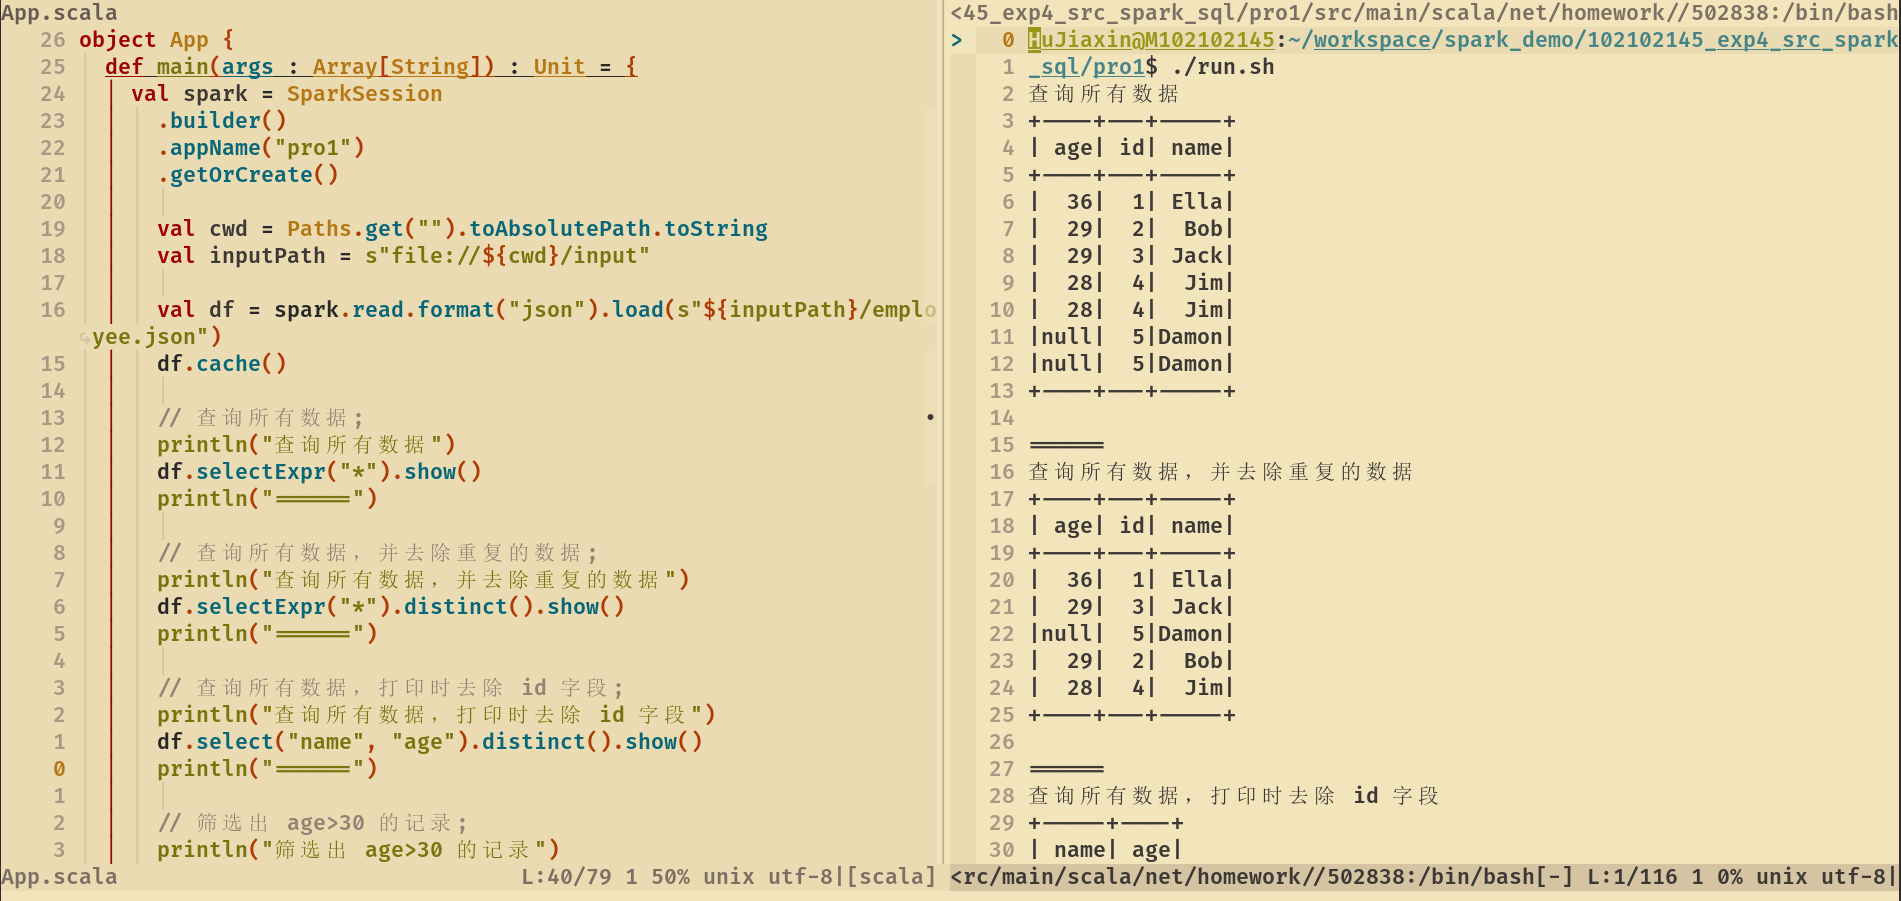
\includegraphics[width=0.95\textwidth]{./figures/1-0.png}
  \end{center}
  \caption{运行结果}
\end{figure}
\begin{figure}[H]
  \begin{center}
    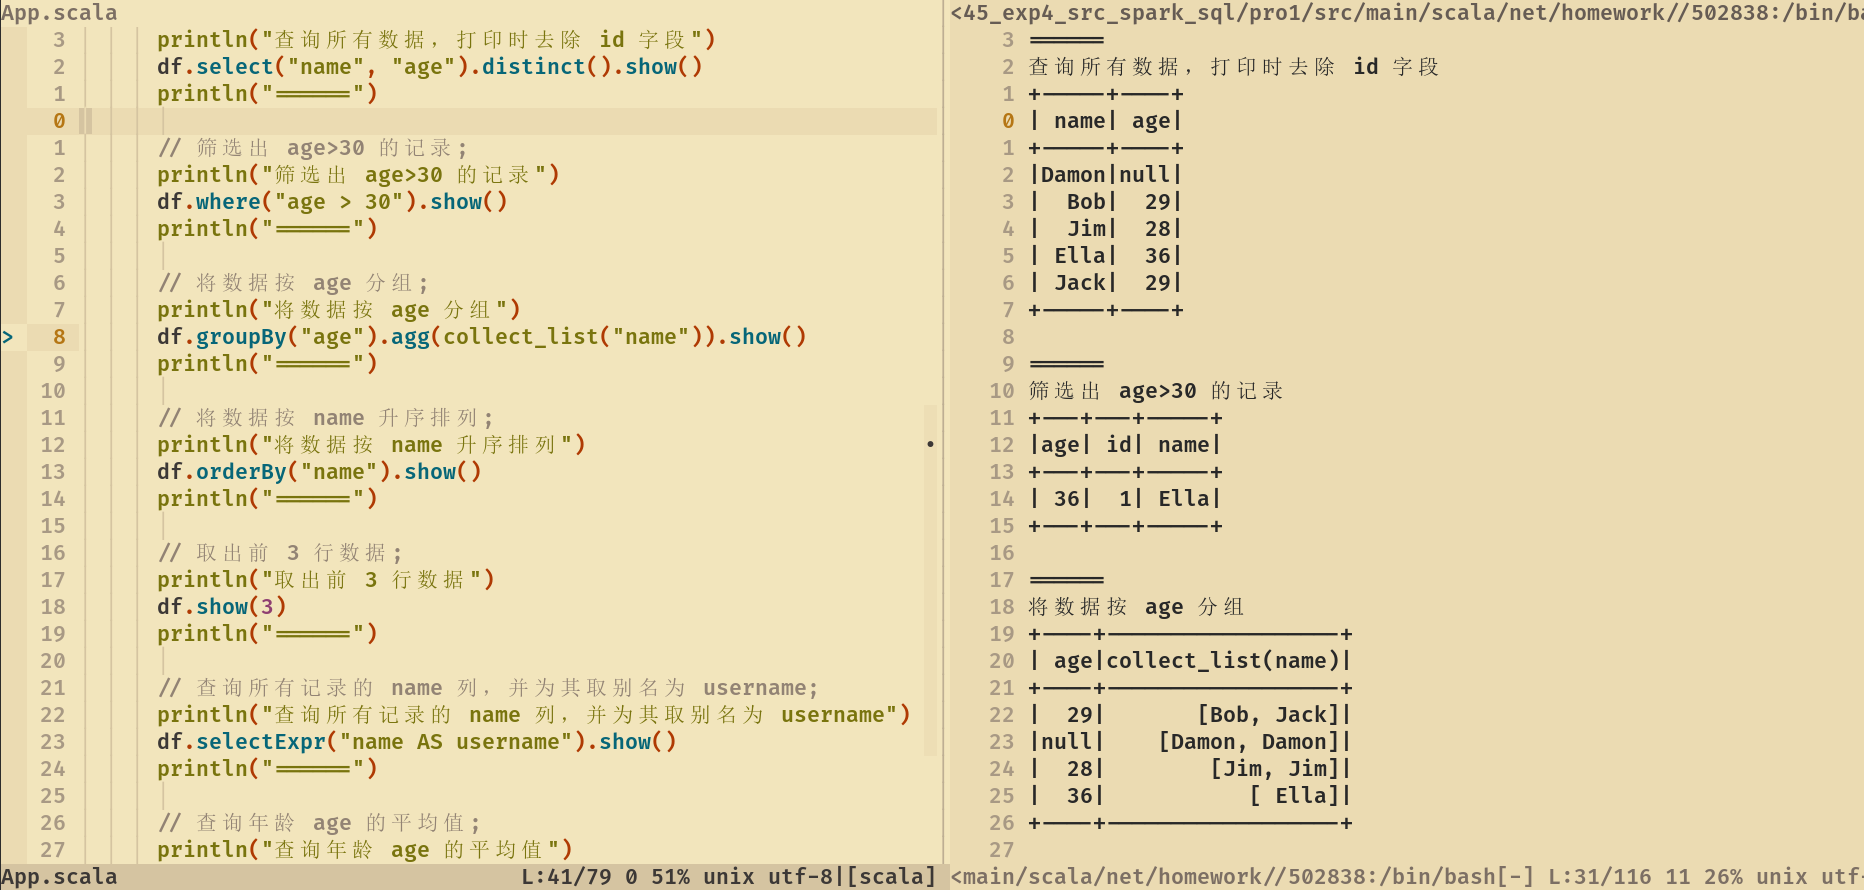
\includegraphics[width=0.95\textwidth]{./figures/1-1.png}
  \end{center}
  \caption{运行结果}
\end{figure}
\begin{figure}[H]
  \begin{center}
    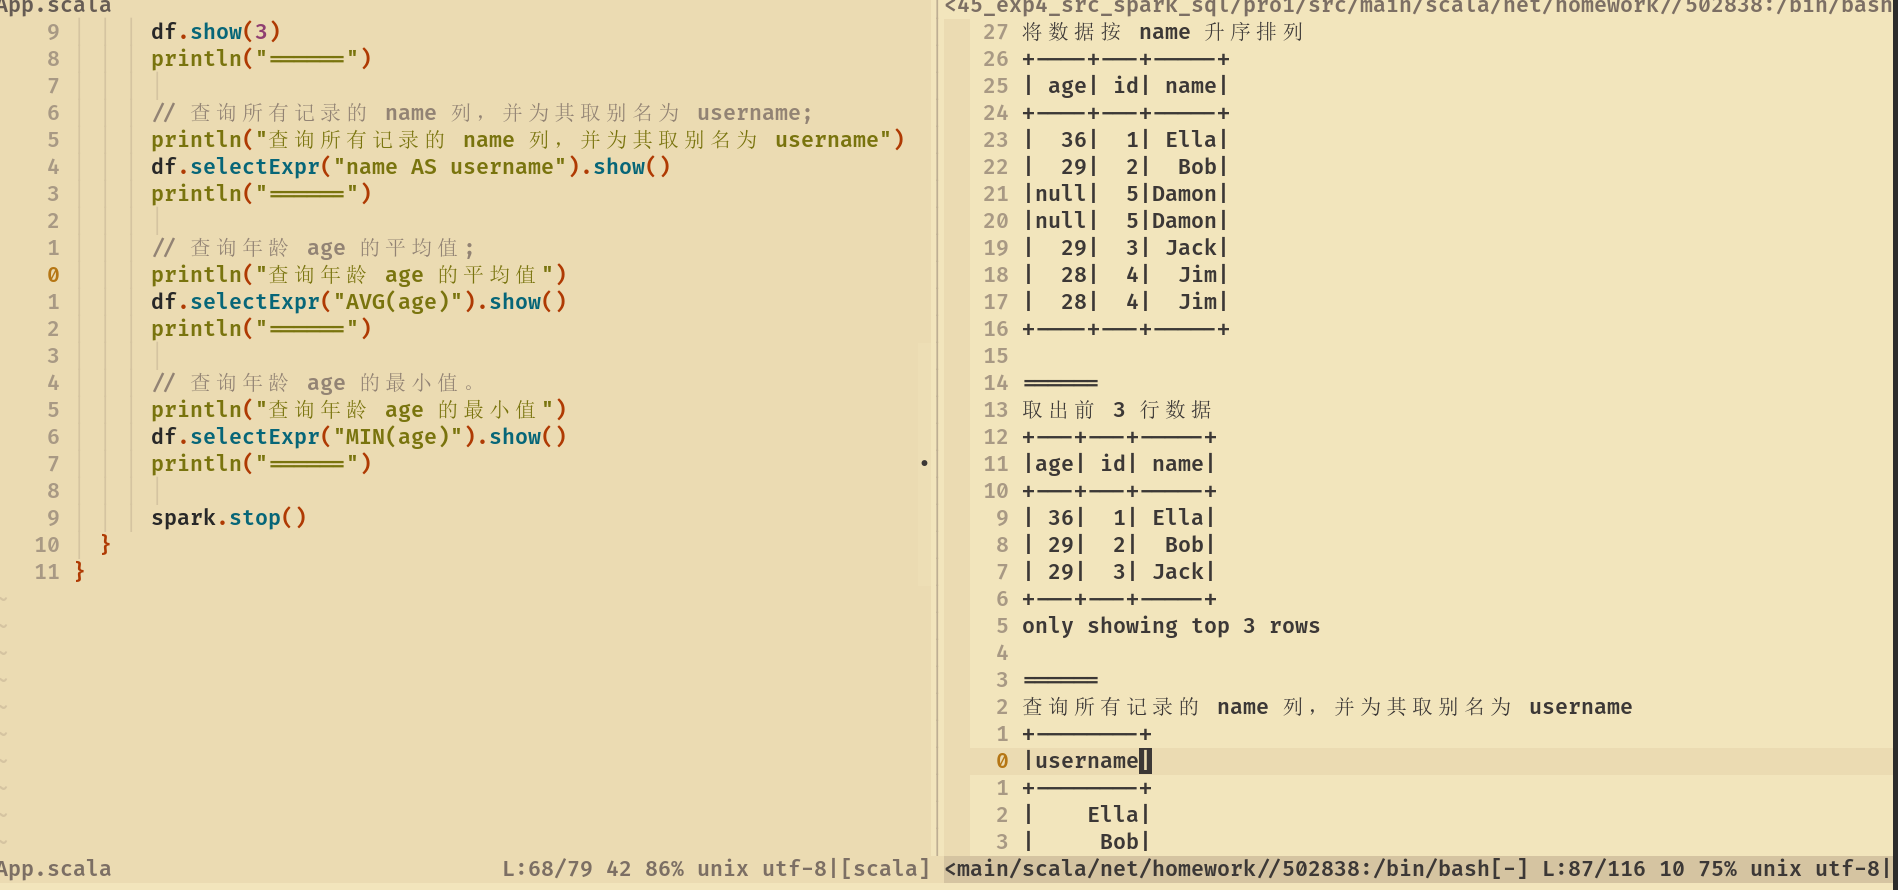
\includegraphics[width=0.95\textwidth]{./figures/1-2.png}
  \end{center}
  \caption{运行结果}
\end{figure}
\begin{figure}[H]
  \begin{center}
    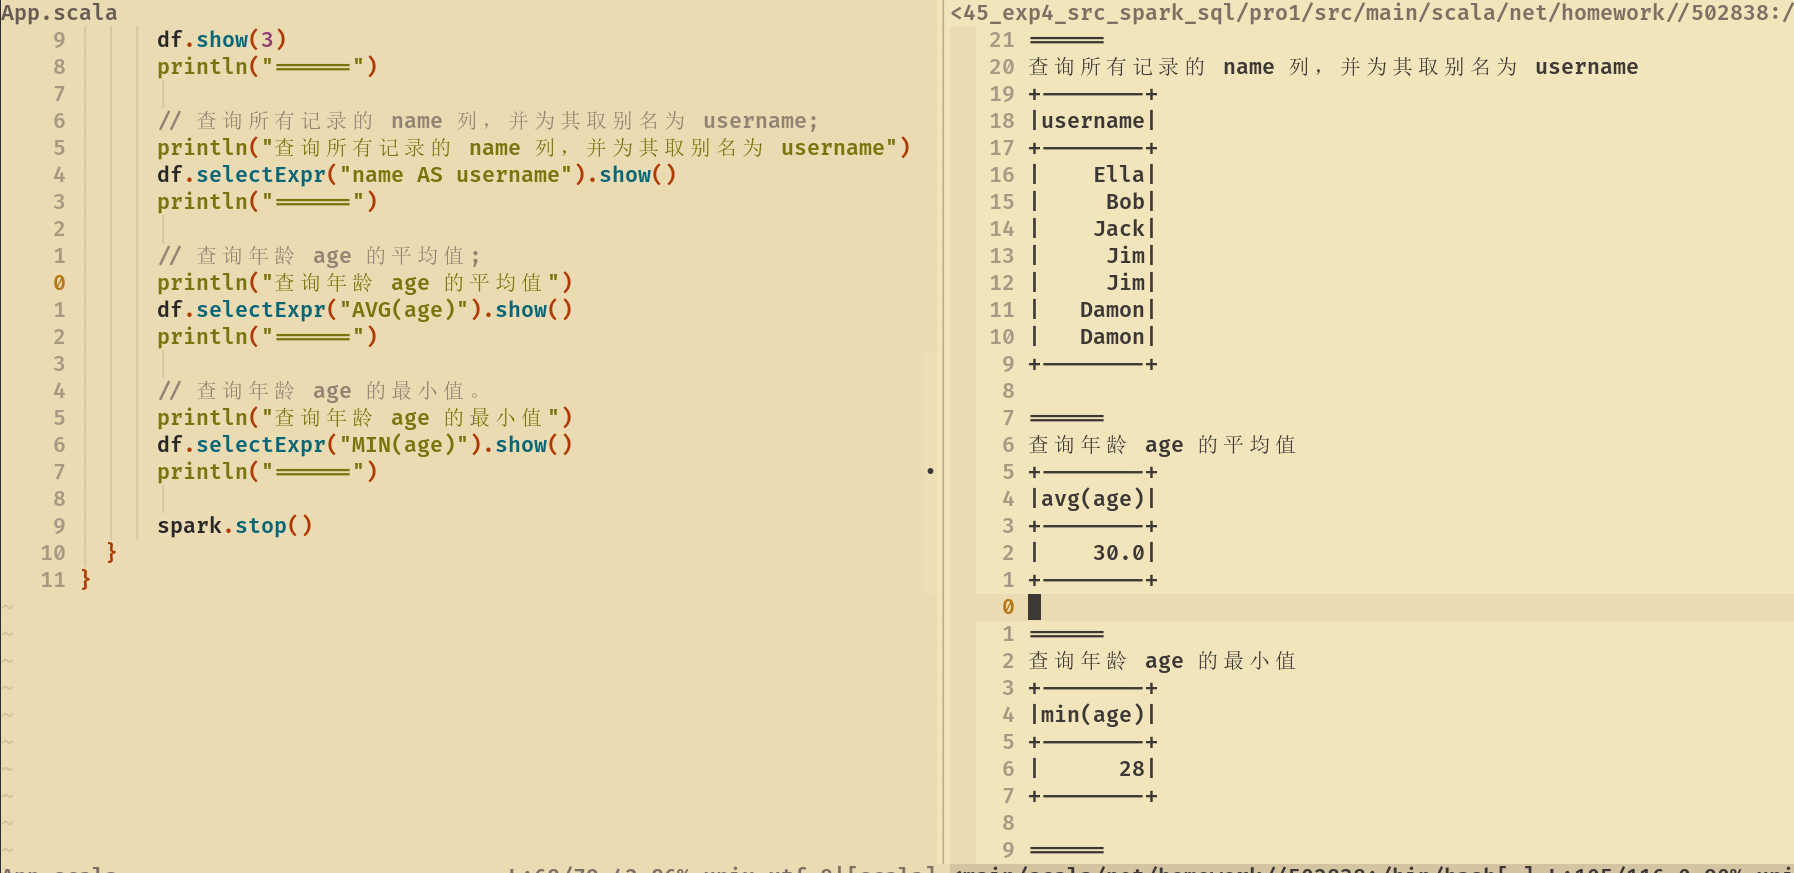
\includegraphics[width=0.95\textwidth]{./figures/1-3.png}
  \end{center}
  \caption{运行结果}
\end{figure}


\subsection{咖啡供应链统计}
\subsubsection{Problem Description}
Coffee Chain.csv 数据字段如下:

\noindent Area Code 区号 \\
Ddate 统计日期 \\
Market 市场位置 \\
Market Size 市场规模 \\
Product 产品 \\
Product Type 产品类别 \\
State 所在州 \\
Type 产品属性 \\
Budget Cogs 预算成本 \\
Budget Margin 预算盈余 \\
Budget Profit 利润预算 \\
Budget Sales 销售预算 \\
Coffee Sales 实际销售 \\
Cogs 实际成本 \\
Inventory 库存 \\
Margin 实际盈余 \\
Marketing 销售量 \\
Number of Records 记录数 \\
Profit 实际利润 \\
Total Expenses 其他成本 \\

\begin{enumerate}
  \item 查看咖啡连锁店的销售量排名,按照销售量降序排列。
  \item 查看咖啡销售量和所在州的关系,按降序排列。
  \item 查询咖啡的平均利润和售价,按平均利润降序排列。
  \item 查询市场规模、市场地域与销售量的关系。按总销量降序排列.
  \item 查询咖啡属性与平均售价、平均利润、销售量与其他成本的关系。
\end{enumerate}

\subsubsection{Code}
\begin{center}
\begin{minted}[xleftmargin=5mm]{scala}
package net.homework

import org.apache.spark.SparkContext._
import org.apache.spark.sql.SparkSession
import org.apache.spark.sql.Row
import org.apache.spark.sql.functions.{desc, expr}

import java.nio.file.Paths

object App {
  def main(args : Array[String]) : Unit = {
    val spark = SparkSession.builder().appName("pro2").getOrCreate()

      val cwd = Paths.get("").toAbsolutePath.toString
      val inputPath = s"file://${cwd}/input"

      val df = spark.read
        .option("header", "true")
        .option("inferSchema", "true")
        .format("csv")
        .load(s"${inputPath}/Coffee_Chain.csv")
      df.cache()

      //df.printSchema()

      // 查看咖啡连锁店的销售量排名,按照销售量降序排列。
      println("查看咖啡连锁店的销售量排名,按照销售量降序排列")
      df.select("product", "marketing")
        .groupBy("product")
        .agg(expr("SUM(marketing) AS number"))
        .orderBy(desc("number"))
        .show()
      println("======")

      // 查看咖啡销售量和所在州的关系,按降序排列。
      println("查看咖啡销售量和所在州的关系,按降序排列")
      df.select("state", "marketing")
        .groupBy("state")
        .agg(expr("SUM(marketing) AS number"))
        .orderBy(desc("number"))
        .show()
      println("======")

      // 查询咖啡的平均利润和售价,按平均利润降序排列。
      println("查询咖啡的平均利润和售价,按平均利润降序排列")
      df.select("product", "coffee sales", "profit")
        .groupBy("product")
        .agg(expr("avg(`coffee sales`)"), expr("avg(profit) as avg_profit"))
        .orderBy(desc("avg_profit"))
        .show()
      println("======")

      // 查询市场规模、市场地域与销售量的关系。按总销量降序排列.
      println("查询市场规模、市场地域与销售量的关系。按总销量降序排列")
      df.select("market", "market size", "coffee sales")
        .groupBy("market", "market size")
        .agg(expr("SUM(`coffee sales`) AS total_sales"))
        .orderBy(desc("total_sales"))
        .show()
      println("======")

      // 查询咖啡属性与平均售价、平均利润、销售量与其他成本的关系。
      println("查询咖啡属性与平均售价、平均利润、销售量与其他成本的关系")
      df.select("type", "profit", "coffee sales",  "total expenses",
        "marketing", "budget sales")
        .groupBy("type")
        .agg(
          expr("AVG(`coffee sales`) AS avg_sales"),
          expr("AVG(profit) AS avg_profit"),
          expr("SUM(`coffee sales`) AS total_sales"),
          expr("AVG(`total expenses`) AS other_cost"))
        .show()
      println("======")

      spark.stop()
  }
}
\end{minted}
\end{center}

\subsubsection{Result}
\begin{figure}[H]
  \begin{center}
    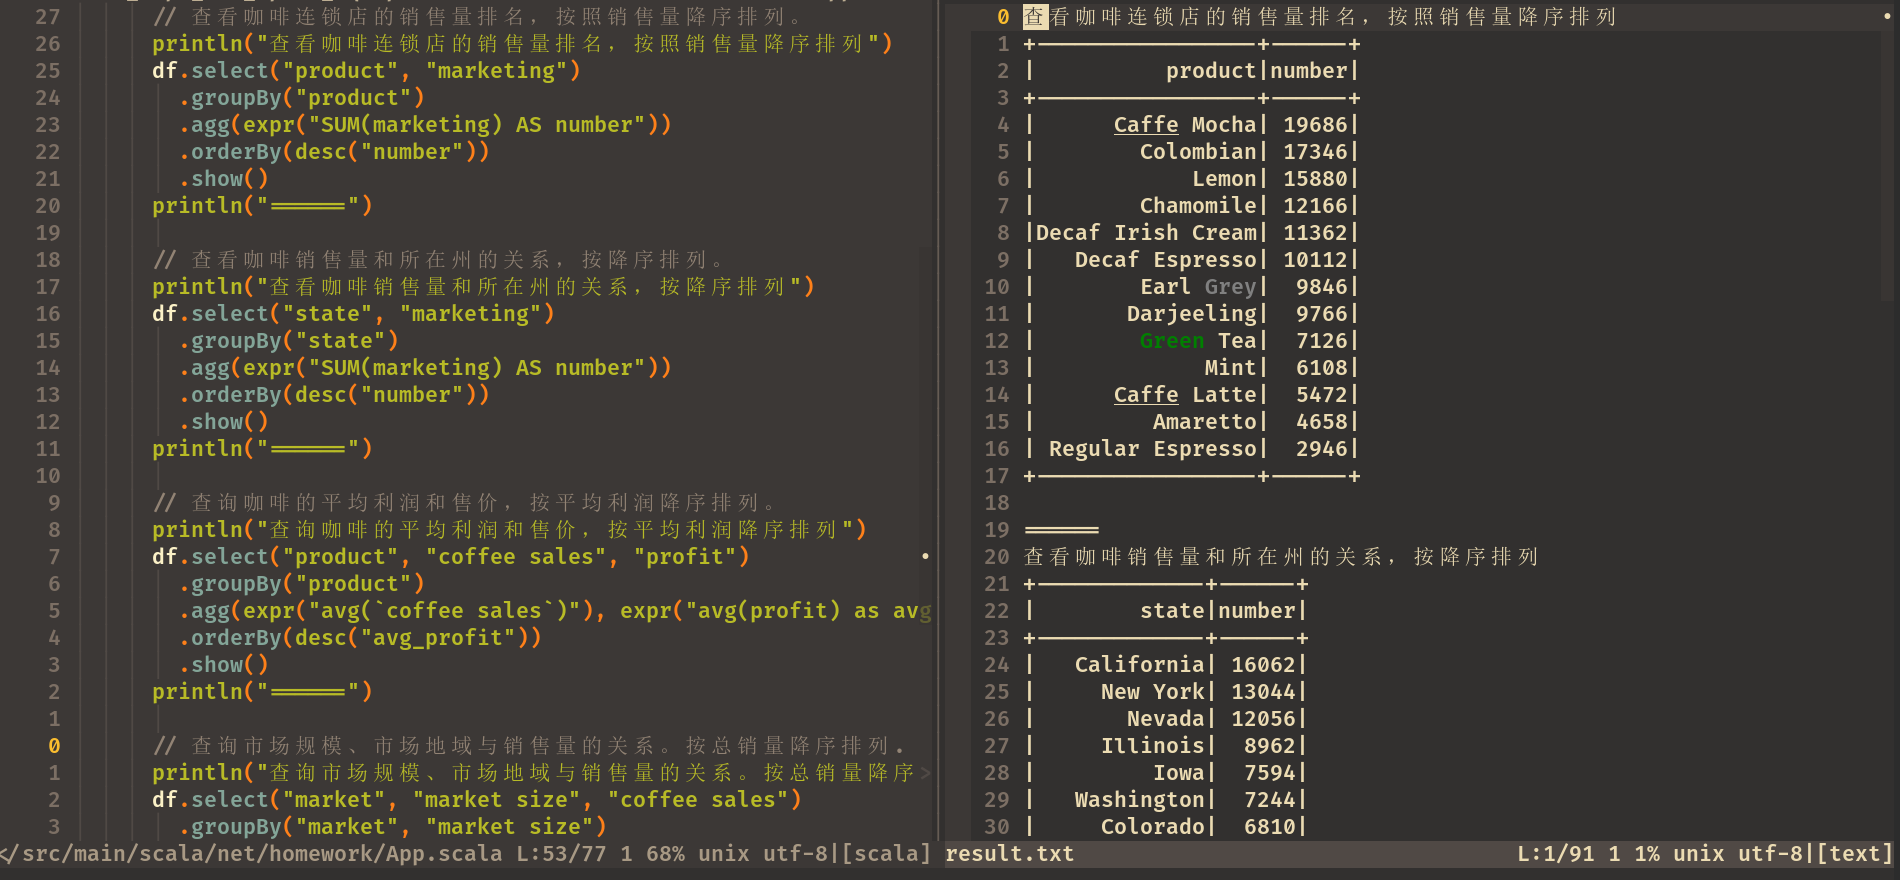
\includegraphics[width=0.95\textwidth]{./figures/2-0.png}
  \end{center}
  \caption{运行结果}
\end{figure}
\begin{figure}[H]
  \begin{center}
    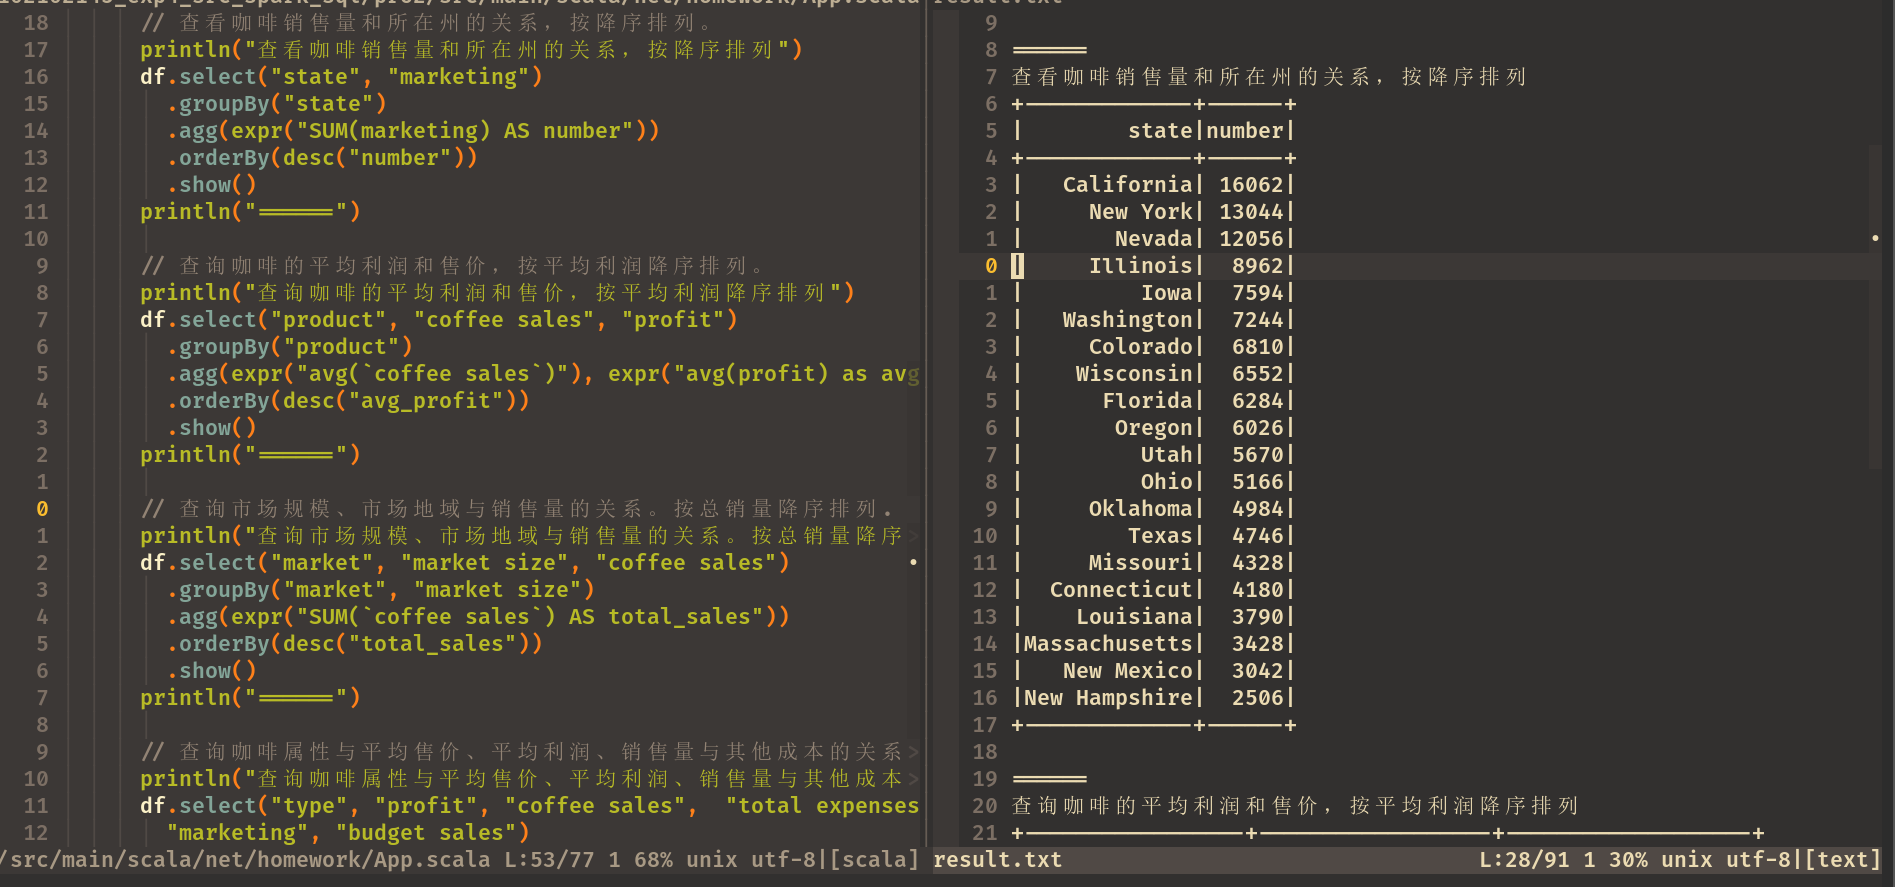
\includegraphics[width=0.95\textwidth]{./figures/2-1.png}
  \end{center}
  \caption{运行结果}
\end{figure}
\begin{figure}[H]
  \begin{center}
    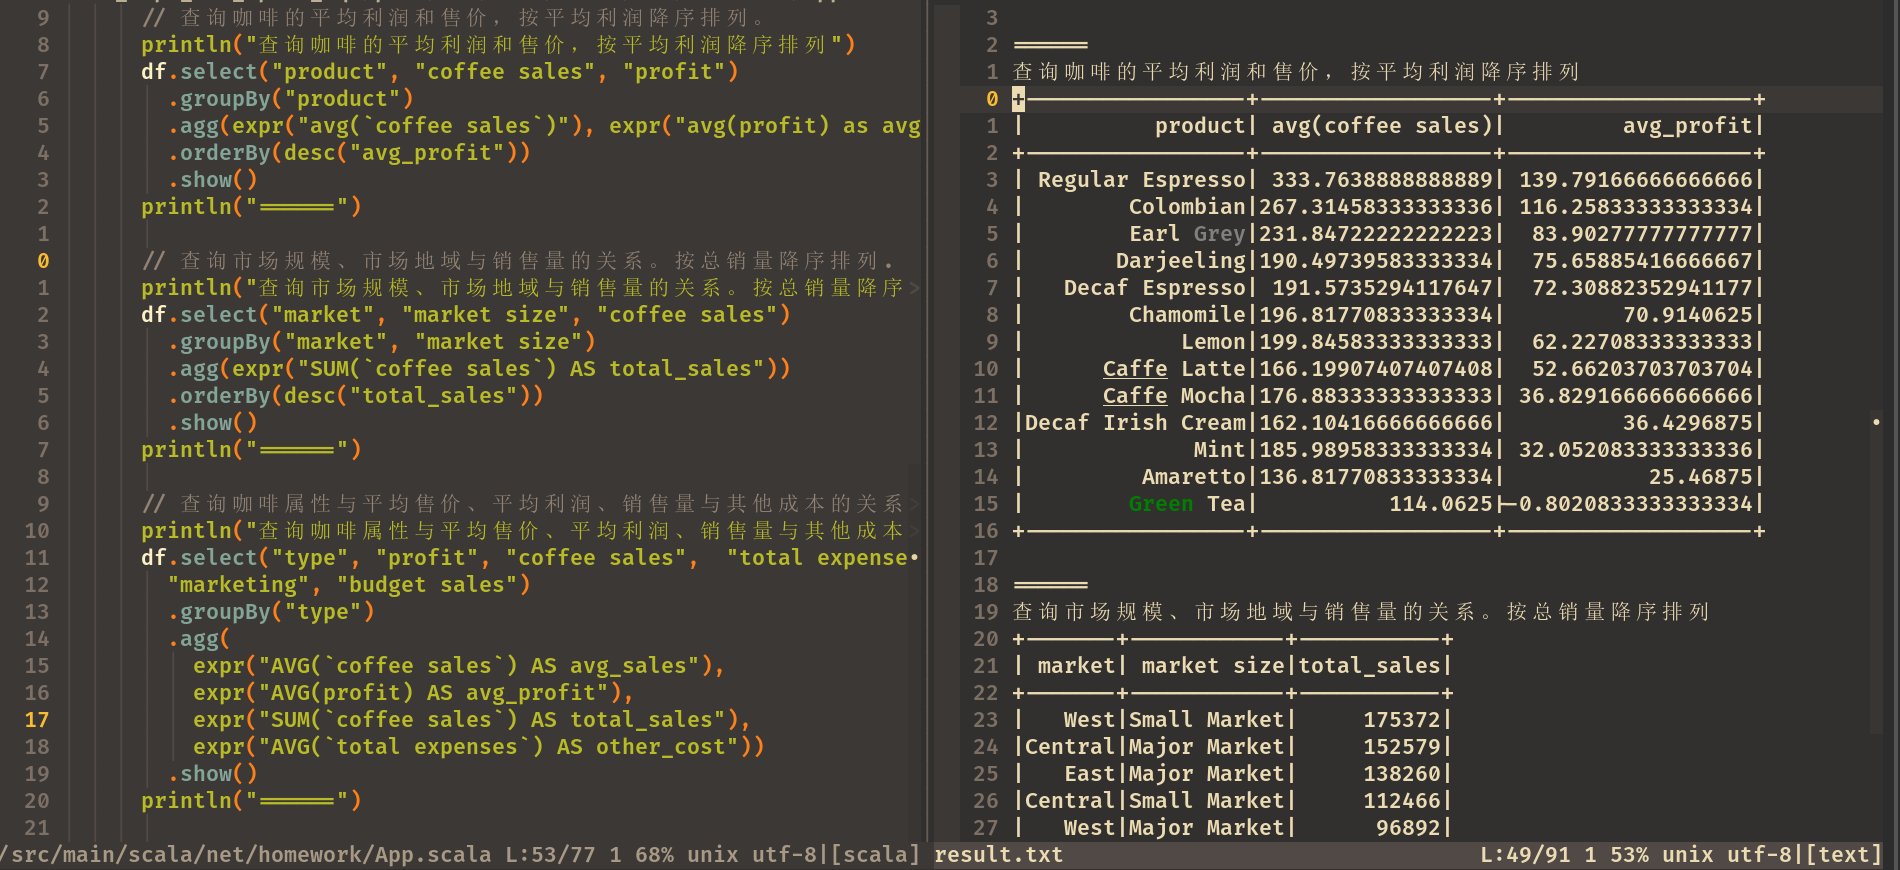
\includegraphics[width=0.95\textwidth]{./figures/2-2.png}
  \end{center}
  \caption{运行结果}
\end{figure}
\begin{figure}[H]
  \begin{center}
    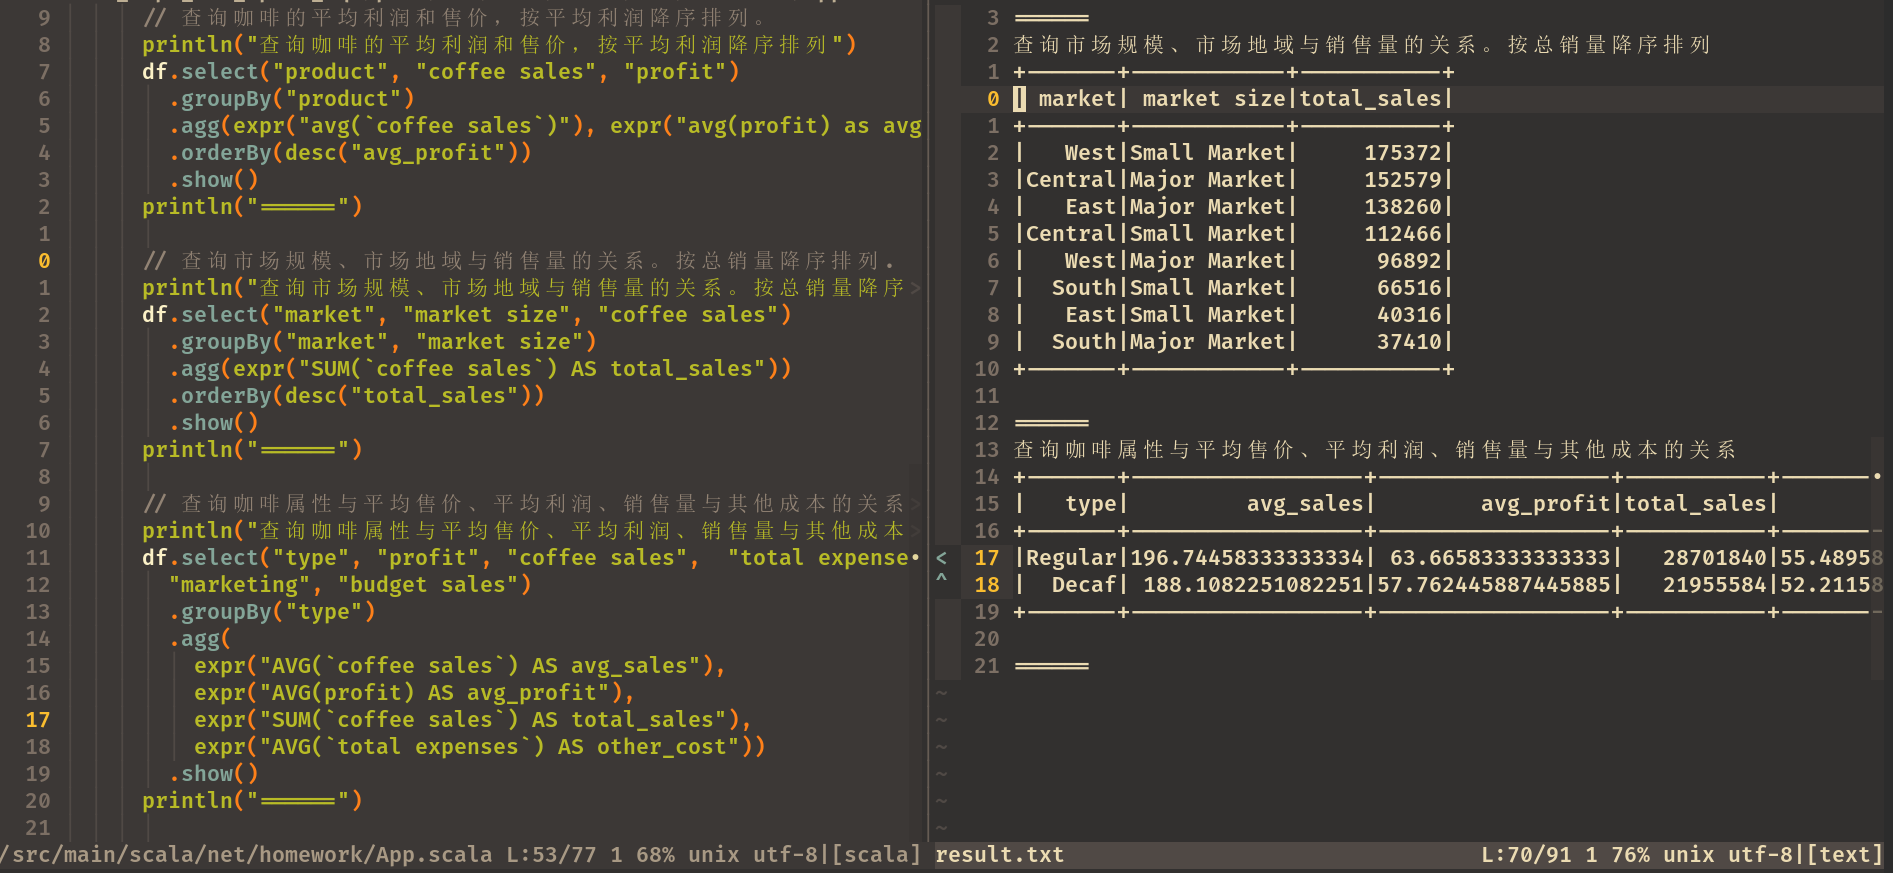
\includegraphics[width=0.95\textwidth]{./figures/2-3.png}
  \end{center}
  \caption{运行结果}
\end{figure}

\subsection{分析校运动会数据}
\subsubsection{Problem Description}
有一份运动会竞赛结果的数据集,其中包括比赛项目、
班级、运动员、成绩和名次,使用 Spark SQL 进行分析。

\begin{enumerate}
  \item 计算平均成绩:
    \begin{itemize}
      \item 计算所有比赛项目的平均成绩
    \end{itemize}
  \item 统计每个班级的名次总数:
    \begin{itemize}
      \item 统计每个班级获得的第一名、第二名和第三名的次数。
      \item 列出获得第一名次数超过 2 次的班级。
    \end{itemize}
  \item 筛选并统计特定项目的成绩:
    \begin{itemize}
      \item 筛选出所有田径项目(如 100 米短跑、200 米短跑)的比赛结果。
      \item 统计在这些田径项目中获得前三名的个人数量。
    \end{itemize}
\end{enumerate}
提示:通过 \code{StructType} 创建模式;利用 \code{spark.read.csv()} 读取数据;使用 \code{createOrReplaceTempView}
创建临时表;使用 \code{filter} 进行过滤,使用 \code{groupby},\code{agg} 进行聚合.

\subsubsection{Code}
\begin{center}
\begin{minted}[xleftmargin=5mm]{scala}
package net.homework

import org.apache.spark.{SparkConf, SparkContext}
import org.apache.spark.SparkContext._
import org.apache.spark.sql.SparkSession
import org.apache.spark.sql.types.{
  StructField, StructType,
  StringType, LongType, DoubleType
}
import org.apache.spark.sql.Row

import java.nio.file.Paths

object App {
  def main(args : Array[String]) : Unit = {
    val spark = SparkSession
      .builder()
      .appName("pro3")
      .getOrCreate()

    val cwd = Paths.get("").toAbsolutePath.toString
    val inputPath = s"file://${cwd}/input"

    val textData = spark
      .sparkContext
      .textFile(s"${inputPath}/运动会数据.txt")
      .filter(
        x => {
          !x.startsWith("比赛") && x.length > 0
      })
    val rddInfo = textData
      .map(
        x => {
          val arr = x.split(",")
          Row(arr(0).trim, arr(1).trim, arr(2).trim,
            arr(3).trim.toDouble, arr(4).trim.toLong)
      })

    val schema = new StructType(Array(
      new StructField("category", StringType),
      new StructField("class", StringType),
      new StructField("player", StringType),
      new StructField("score", DoubleType),
      new StructField("rank", LongType)
    ))
    //rddInfo.foreach(println)

    val dfInfo = spark.createDataFrame(rddInfo, schema)
    //dfInfo.show()

    dfInfo.createOrReplaceTempView("info")

    // 计算所有比赛项目的平均成绩
    println("计算所有比赛项目的平均成绩:")
    spark
      .sql("""SELECT ROUND(AVG(score), 2) AS Avg_Score
        FROM info
        GROUP BY category""")
      .show()
    println("=======")

    // 统计每个班级获得的第一名、第二名和第三名的次数。
    println("统计每个班级获得的第一名、第二名和第三名的次数:")
    spark
      .sql("""SELECT info.class, COUNT(*) AS First_Num
        FROM info
        WHERE rank=1
        GROUP BY class""")
      .show()
    spark
      .sql("""SELECT info.class, COUNT(*) AS Second_Num
        FROM info
        WHERE rank=2
        GROUP BY class""")
      .show()
    spark
      .sql("""SELECT info.class, COUNT(*) AS Third_Num
        FROM info
        WHERE rank=3
        GROUP BY class""")
      .show()
    println("========")

    // 列出获得第一名次数超过 2 次的班级。
    println("列出获得第一名次数超过 2 次的班级:")
    spark
      .sql("""SELECT info.class, COUNT(*) AS Num
        FROM info
        WHERE rank=1
        GROUP BY class having count(*)>2""")
      .show()
    println("========")

    // 筛选出所有田径项目(如 100 米短跑、200 米短跑)的比赛结果。
    println("筛选出所有田径项目(如 100 米短跑、200 米短跑)的比赛结果:")
    spark
      .sql("""SELECT *
        FROM info
        ORDER BY category, rank""")
      .show()

    // 统计在这些田径项目中获得前三名的个人数量。
    println("统计在这些田径项目中获得前三名的个人数量:")
    spark
      .sql("""SELECT DISTINCT COUNT(*)
        FROM info
        WHERE rank<=3""")
      .show()


    spark.stop()
  }
}
\end{minted}
\end{center}

\subsubsection{Result}
\begin{figure}[H]
  \begin{center}
    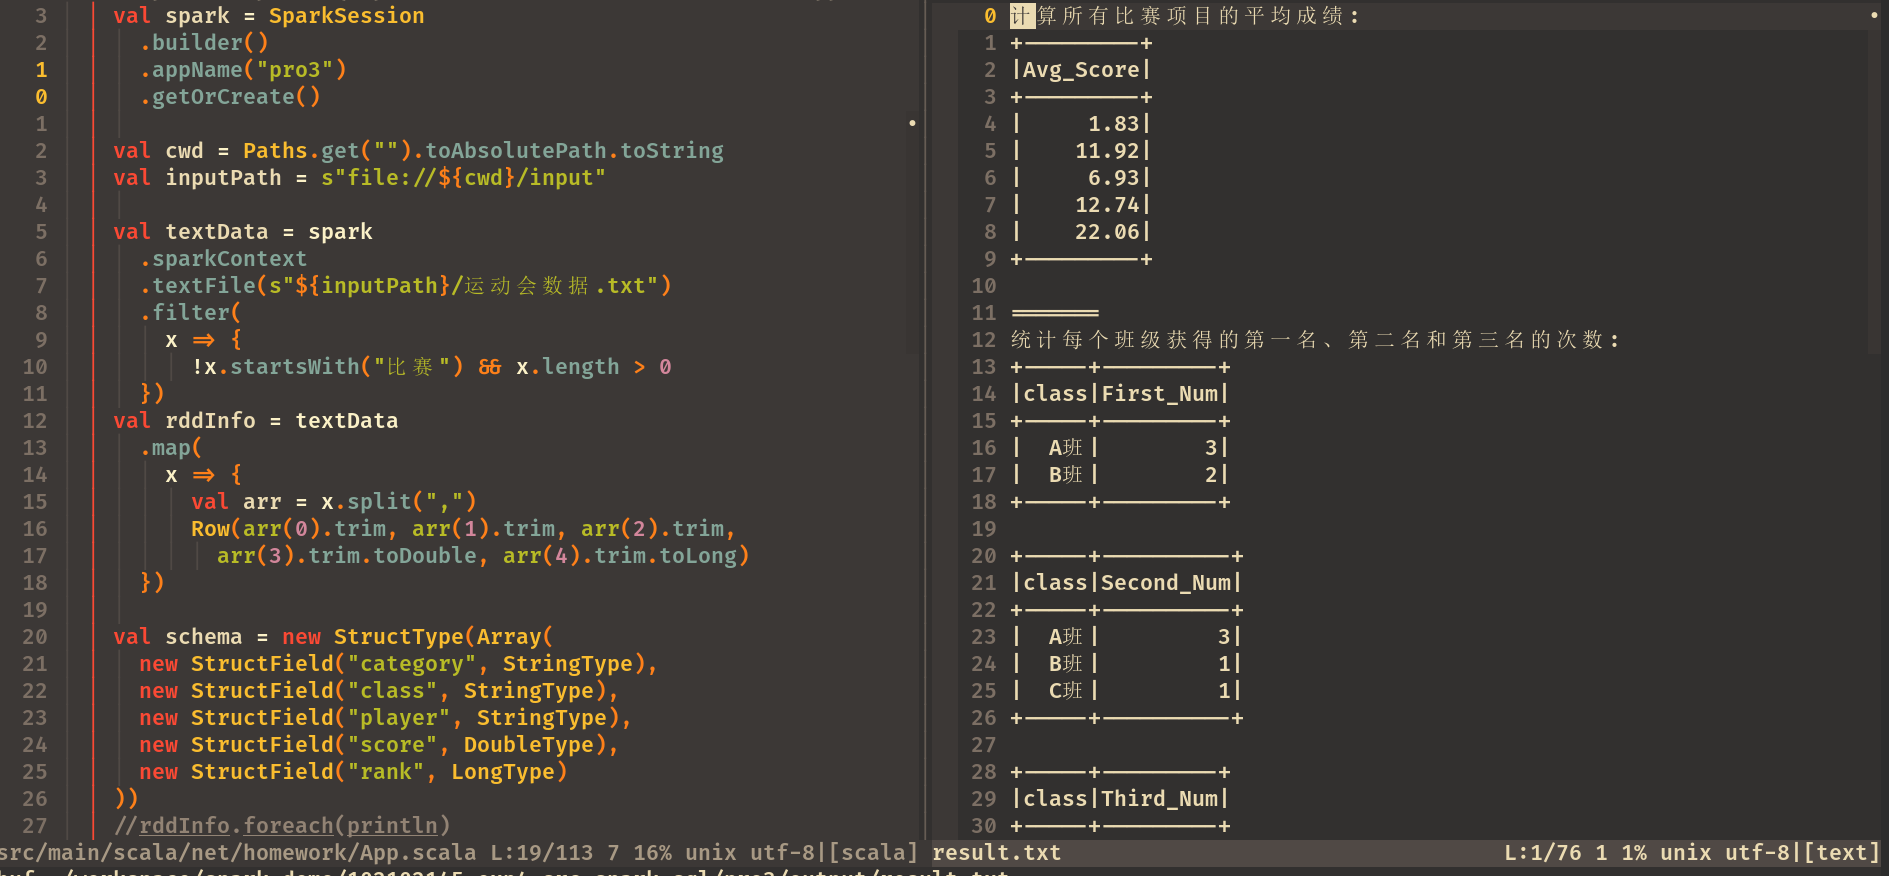
\includegraphics[width=0.95\textwidth]{./figures/3-0.png}
  \end{center}
  \caption{运行结果}
\end{figure}
\begin{figure}[H]
  \begin{center}
    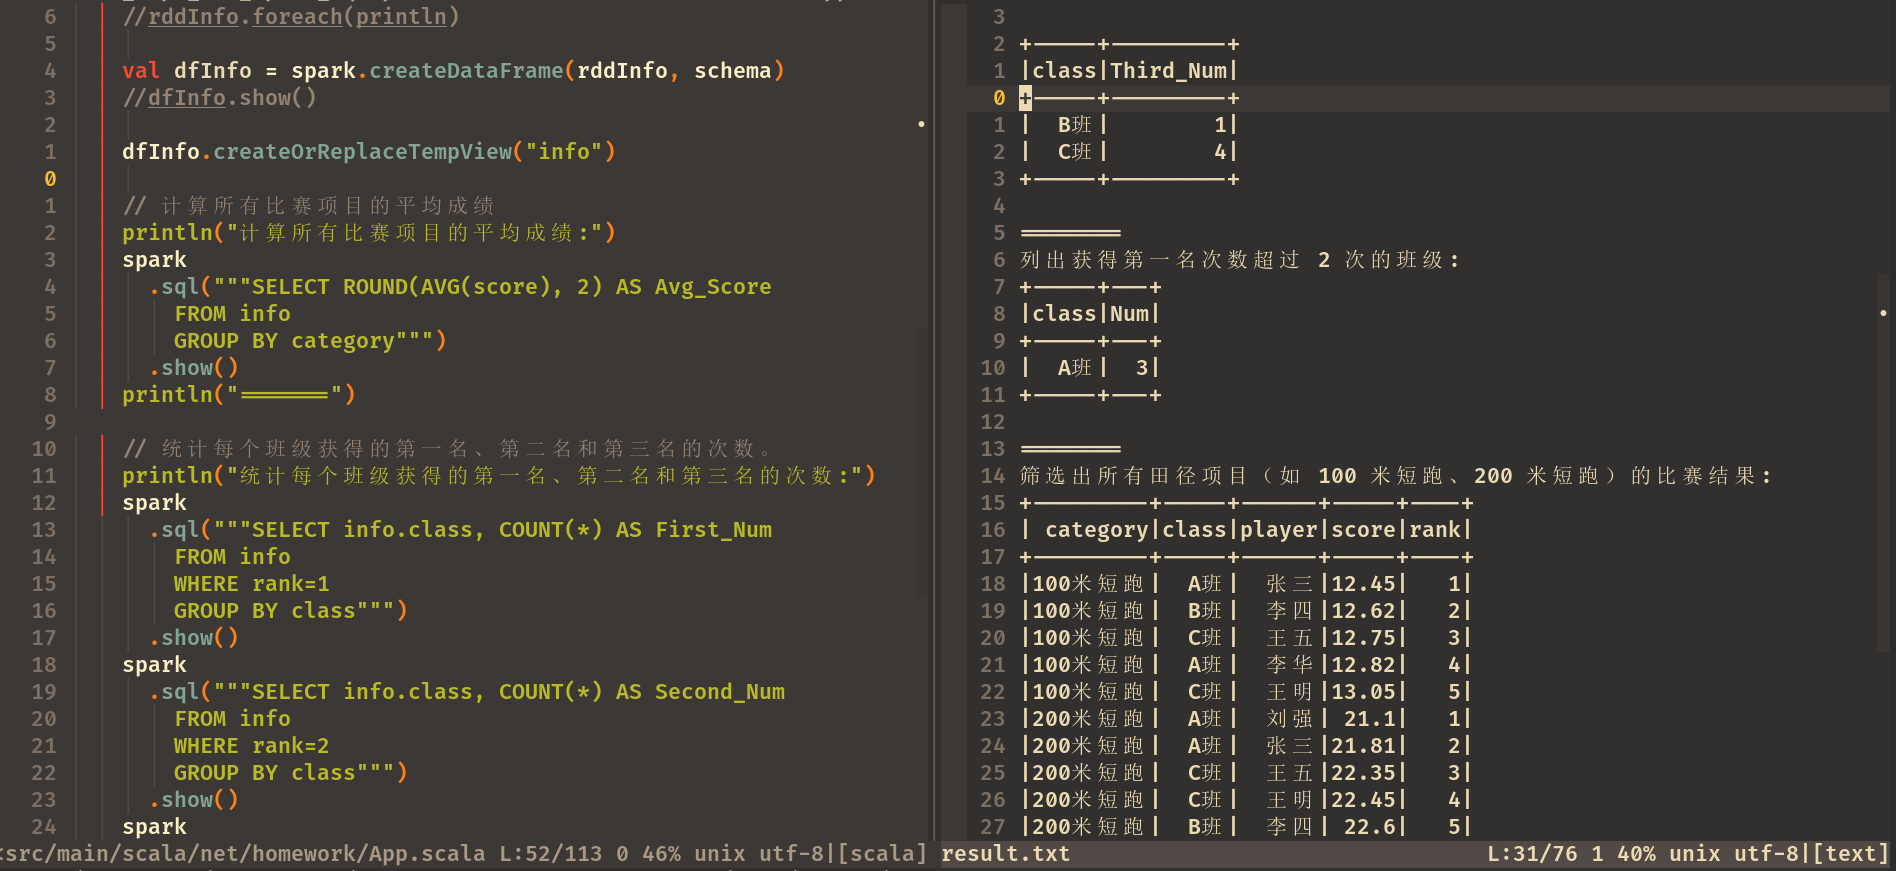
\includegraphics[width=0.95\textwidth]{./figures/3-1.png}
  \end{center}
  \caption{运行结果}
\end{figure}
\begin{figure}[H]
  \begin{center}
    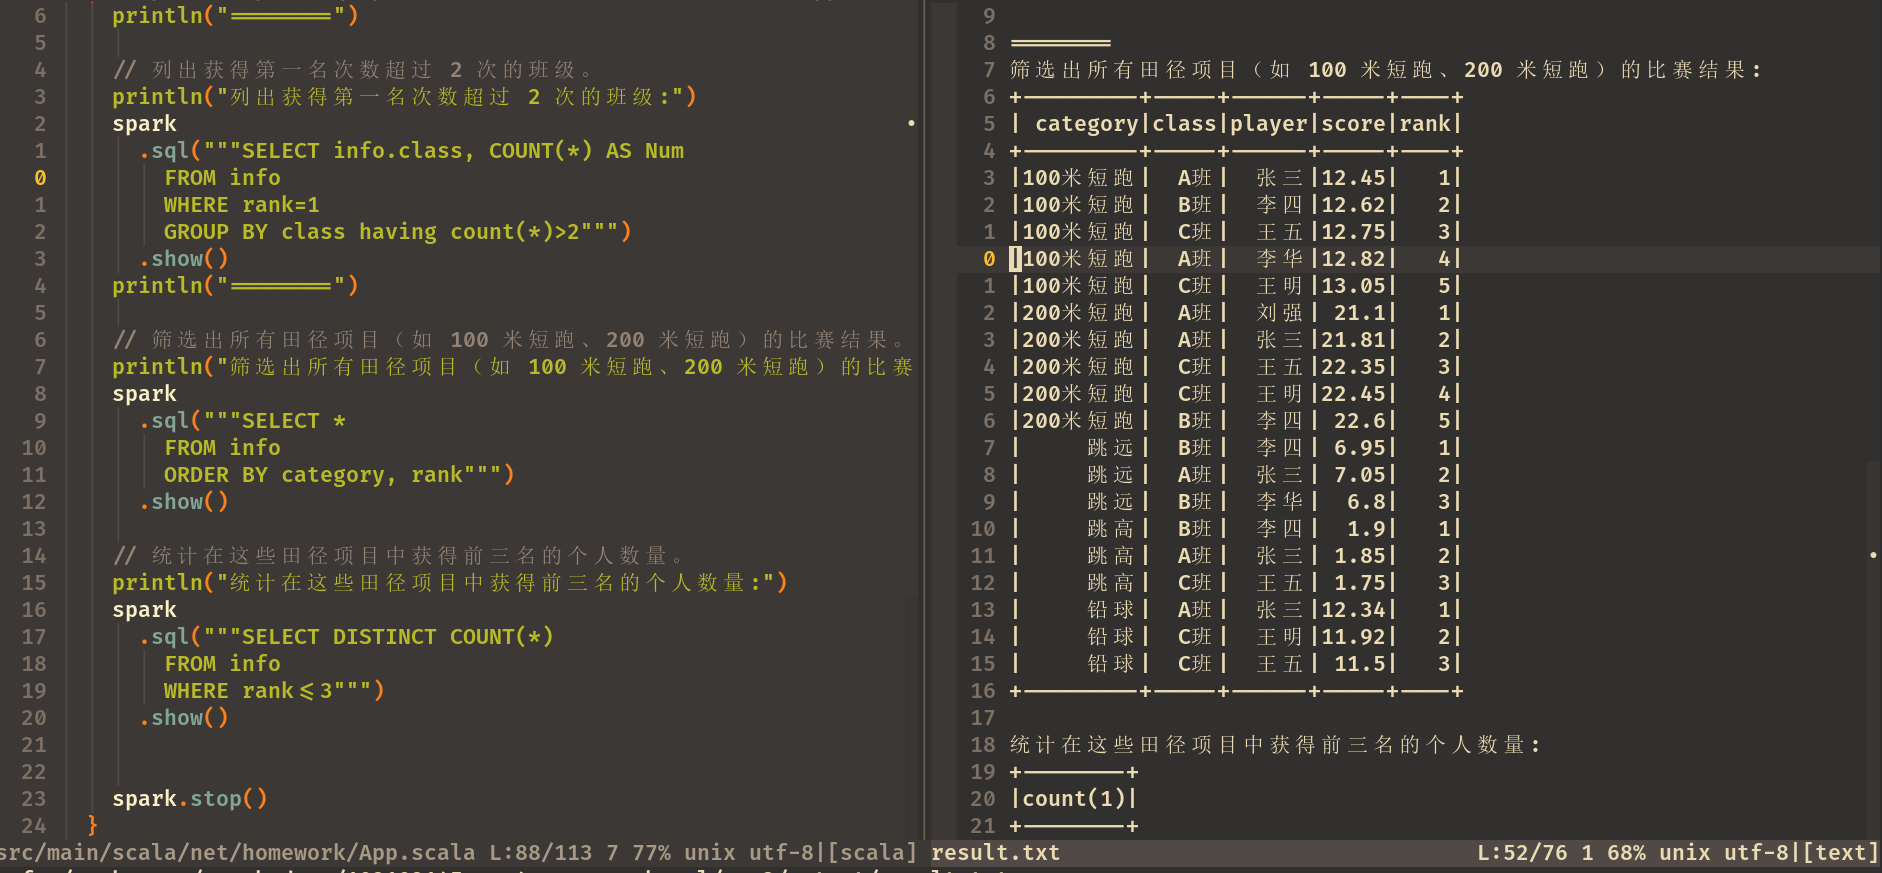
\includegraphics[width=0.95\textwidth]{./figures/3-2.png}
  \end{center}
  \caption{运行结果}
\end{figure}

\section{出现的问题及其解决方案}
没有问题.
\end{document}
